% Author: Nikita Moiseev <xmoise01@stud.fit.vutbr.cz>
% Author: Elena Marochkina <xmaroc00@stud.fit.vutbr.cz>
% Author: Nikita Pasynkov <xpasyn0034@stud.fit.vutbr.cz>


\documentclass[a4paper, 11pt]{article}

\usepackage[czech]{babel}
\usepackage[utf8]{inputenc}
\usepackage{geometry}
\usepackage{placeins}
\geometry{verbose,a4paper,tmargin=2cm,bmargin=2cm,lmargin=2.5cm,rmargin=1.5cm}
\usepackage{times}
\renewcommand{\baselinestretch}{1.5}
\usepackage{geometry}
\usepackage{verbatim}
\usepackage{enumitem}
\usepackage{graphicx} % insert picture
\usepackage[unicode]{hyperref}
\usepackage[table,xcdraw]{xcolor}
\documentclass[xcolor=table]{beamer}
\hypersetup{
	colorlinks = false,
	hypertexnames = false,
	citecolor = blue
}
\usepackage{pdflscape}

\begin{document}
	%% Title page %%
	\begin{titlepage}
		\begin{center}
			\includegraphics[width=0.77\linewidth]{fit_logo.png} \\

			\vspace{\stretch{0.382}}

			\Huge{Zpráva o návrhu} \\
			\Huge{\textbf{Aplikace Lékárnička} \\
			\vspace{\stretch{0.7}}
		\end{center}

		\begin{minipage}{0.4 \textwidth}
			{\Large \today}
		\end{minipage}
		\hfill
		\begin{minipage}[r]{0.6 \textwidth}
			\Large
			\begin{tabular}{l l l}
				\textbf{Nikita Moiseev} & \textbf{(xmoise01)} \\
				Elena Marochkina & (xmaroc00) \\
				Nikita Pasynkov & (xpasyn00) \\
			\end{tabular}
		\end{minipage}
	\end{titlepage}



	% Obsah %
	\pagenumbering{roman}
	\setcounter{page}{1}
	\tableofcontents
	\clearpage



	% Úvod %
	\pagenumbering{arabic}
	\setcounter{page}{1}

	\section{Téma}
Jako téma projektu jsme zvolili vytvoření aplikace \textbf{Lékárnička} pro platformu iOS.

Aplikace \textbf{Lékárnička} pomáhá uživateli s následujícím:
\begin{itemize}
  \item Organizace lékárniček na různých místech: v práci, doma, na chatě, v autě, lékárnička na cesty.
  \item Sledování dat expirace léků v lékárničce
  \item Sledování dostupnosti léků v lékárničce
  \item Získání informací o způsobu odběru léků, likvidaci a výrobci
\end{itemize}

	% Návrh a implementace %
	\section{Průzkum uživatelských potřeb}

	\subsection{Dotazník}
Jako testovací platformu jsme použili Google Forms.

Dotazník se skládal z následujících otázek a možných odpovědí.
\begin{enumerate}
\item Máte doma lékárničku?
\begin{itemize}
\item Ano
\item No
\end{itemize}
\item Jak často kontrolujete datum spotřeby svých léků?
\begin{itemize}
    \item Jednou týdně
    \item Jednou měsíčně
    \item Jednou za tři měsíce
    \item Pololetně
    \item Jednou za rok
\end{itemize}
\item Jak často kupujete léky??
\begin{itemize}
    \item Jednou týdně
    \item Jednou měsíčně
    \item Jednou za tři měsíce
    \item Pololetně
    \item Jednou za rok
\end{itemize}
\item Stalo se vám někdy, že jste vyhodili léky, protože vypršela doba jejich spotřeby?
\begin{itemize}
\item Ano
\item No
\end{itemize}
\item Stává se vám, že si v lékárně koupíte léky, které už máte v lékárničce?
\begin{itemize}
\item Ano
\item No
\end{itemize}
\item Chtěli byste používat aplikaci, která vám pomůže uspořádat lékárničku?
\begin{itemize}
\item Ano
\item No
\end{itemize}
\item Jaké funkce byste v takové aplikaci rádi viděli??
\begin{itemize}
\item Sledování data expirace
\item Způsob uchovávání léků
\item Způsob použití léků
\item Získání informací o výrobci léku
\item Jak správně likvidovat léky
\item Sledování množství léčiv v lékárničce
\end{itemize}
\end{enumerate}

\textbf {Respondenti}: převážnou část respondentů tvořili studenti různých oborů.

\textbf {Výsledky průzkumu}

Stručně řečeno, údaje z dotazníku odhalují u 19 respondentů pohled na návyky managementu léků a vnímavost k aplikacím organizace léků. Zde jsou hlavní zjištění:

\begin{enumerate}
\item \textbf{Lékárnička}

Většina respondentů (15 z 19) má doma lékárničku, což naznačuje, že udržování zásob léků je mezi respondenty běžné.

\item \textbf {Frekvence kontroly dat vypršení platnosti}

Návyky respondentů při kontrole data expirace svých léků se liší. Většina kontroluje data expirace jednou za tři měsíce (11 z 19), zatímco jiní tak činí pololetně (2 z 19) nebo jednou ročně (6 z 19).

\item \textbf {Likvidace léků s prošlou dobou použitelnosti}

Přibližně polovina respondentů (9 z 19) uvádí, že našla léky s prošlou dobou použitelnosti, což znamená, že chápou důležitost používání bezpečných a účinných léků. Druhá polovina (10 z 19) nenašla ve své lékárničce žádné prošlé léky.

\item \textbf {Nákup duplicitních léků}

Malý počet respondentů (4 z 19) přiznává, že kupuje duplikáty léků, které již mají ve své lékárničce, zatímco většina se této praxi nevěnuje.

\item \textbf {Zájem o používání aplikace pro správu léků}

Značná většina respondentů (13 z 19) vyjádřila přání používat aplikaci Lékárnička, která by jim pomohla spravovat jejich lékárničku.

\item \textbf {Vlastnosti aplikace}

Mezi běžné požadované funkce aplikace organizace léků patří sledování data expirace léků a poskytování pokynů, jak léky používat.
\end{enumerate}

\textbf {Závěr}
Údaje naznačují, že většina respondentů se aktivně podílí na správě svých zásob léků a projevuje proaktivní přístup k bezpečnosti léků. Mají tendenci pravidelně kontrolovat datum spotřeby a značná část vyhazuje prošlé léky. Zájem o použití aplikace organizace léků demonstruje potenciál technologie, která by tomuto procesu pomohla.

Existují však různé úrovně odhodlání kontrolovat data expirace a likvidovat prošlé léky, což naznačuje prostor pro vzdělávání a informovanost o bezpečných léčebných postupech. Celkově tato zjištění podtrhují důležitost managementu léků a zdůrazňují příležitost pro vývoj uživatelsky přívětivých aplikací organizace léků, které dále pomáhají jednotlivcům udržovat bezpečnou a organizovanou lékárničku.

\newpage
\begin{figure}[!ht]
		\centering
		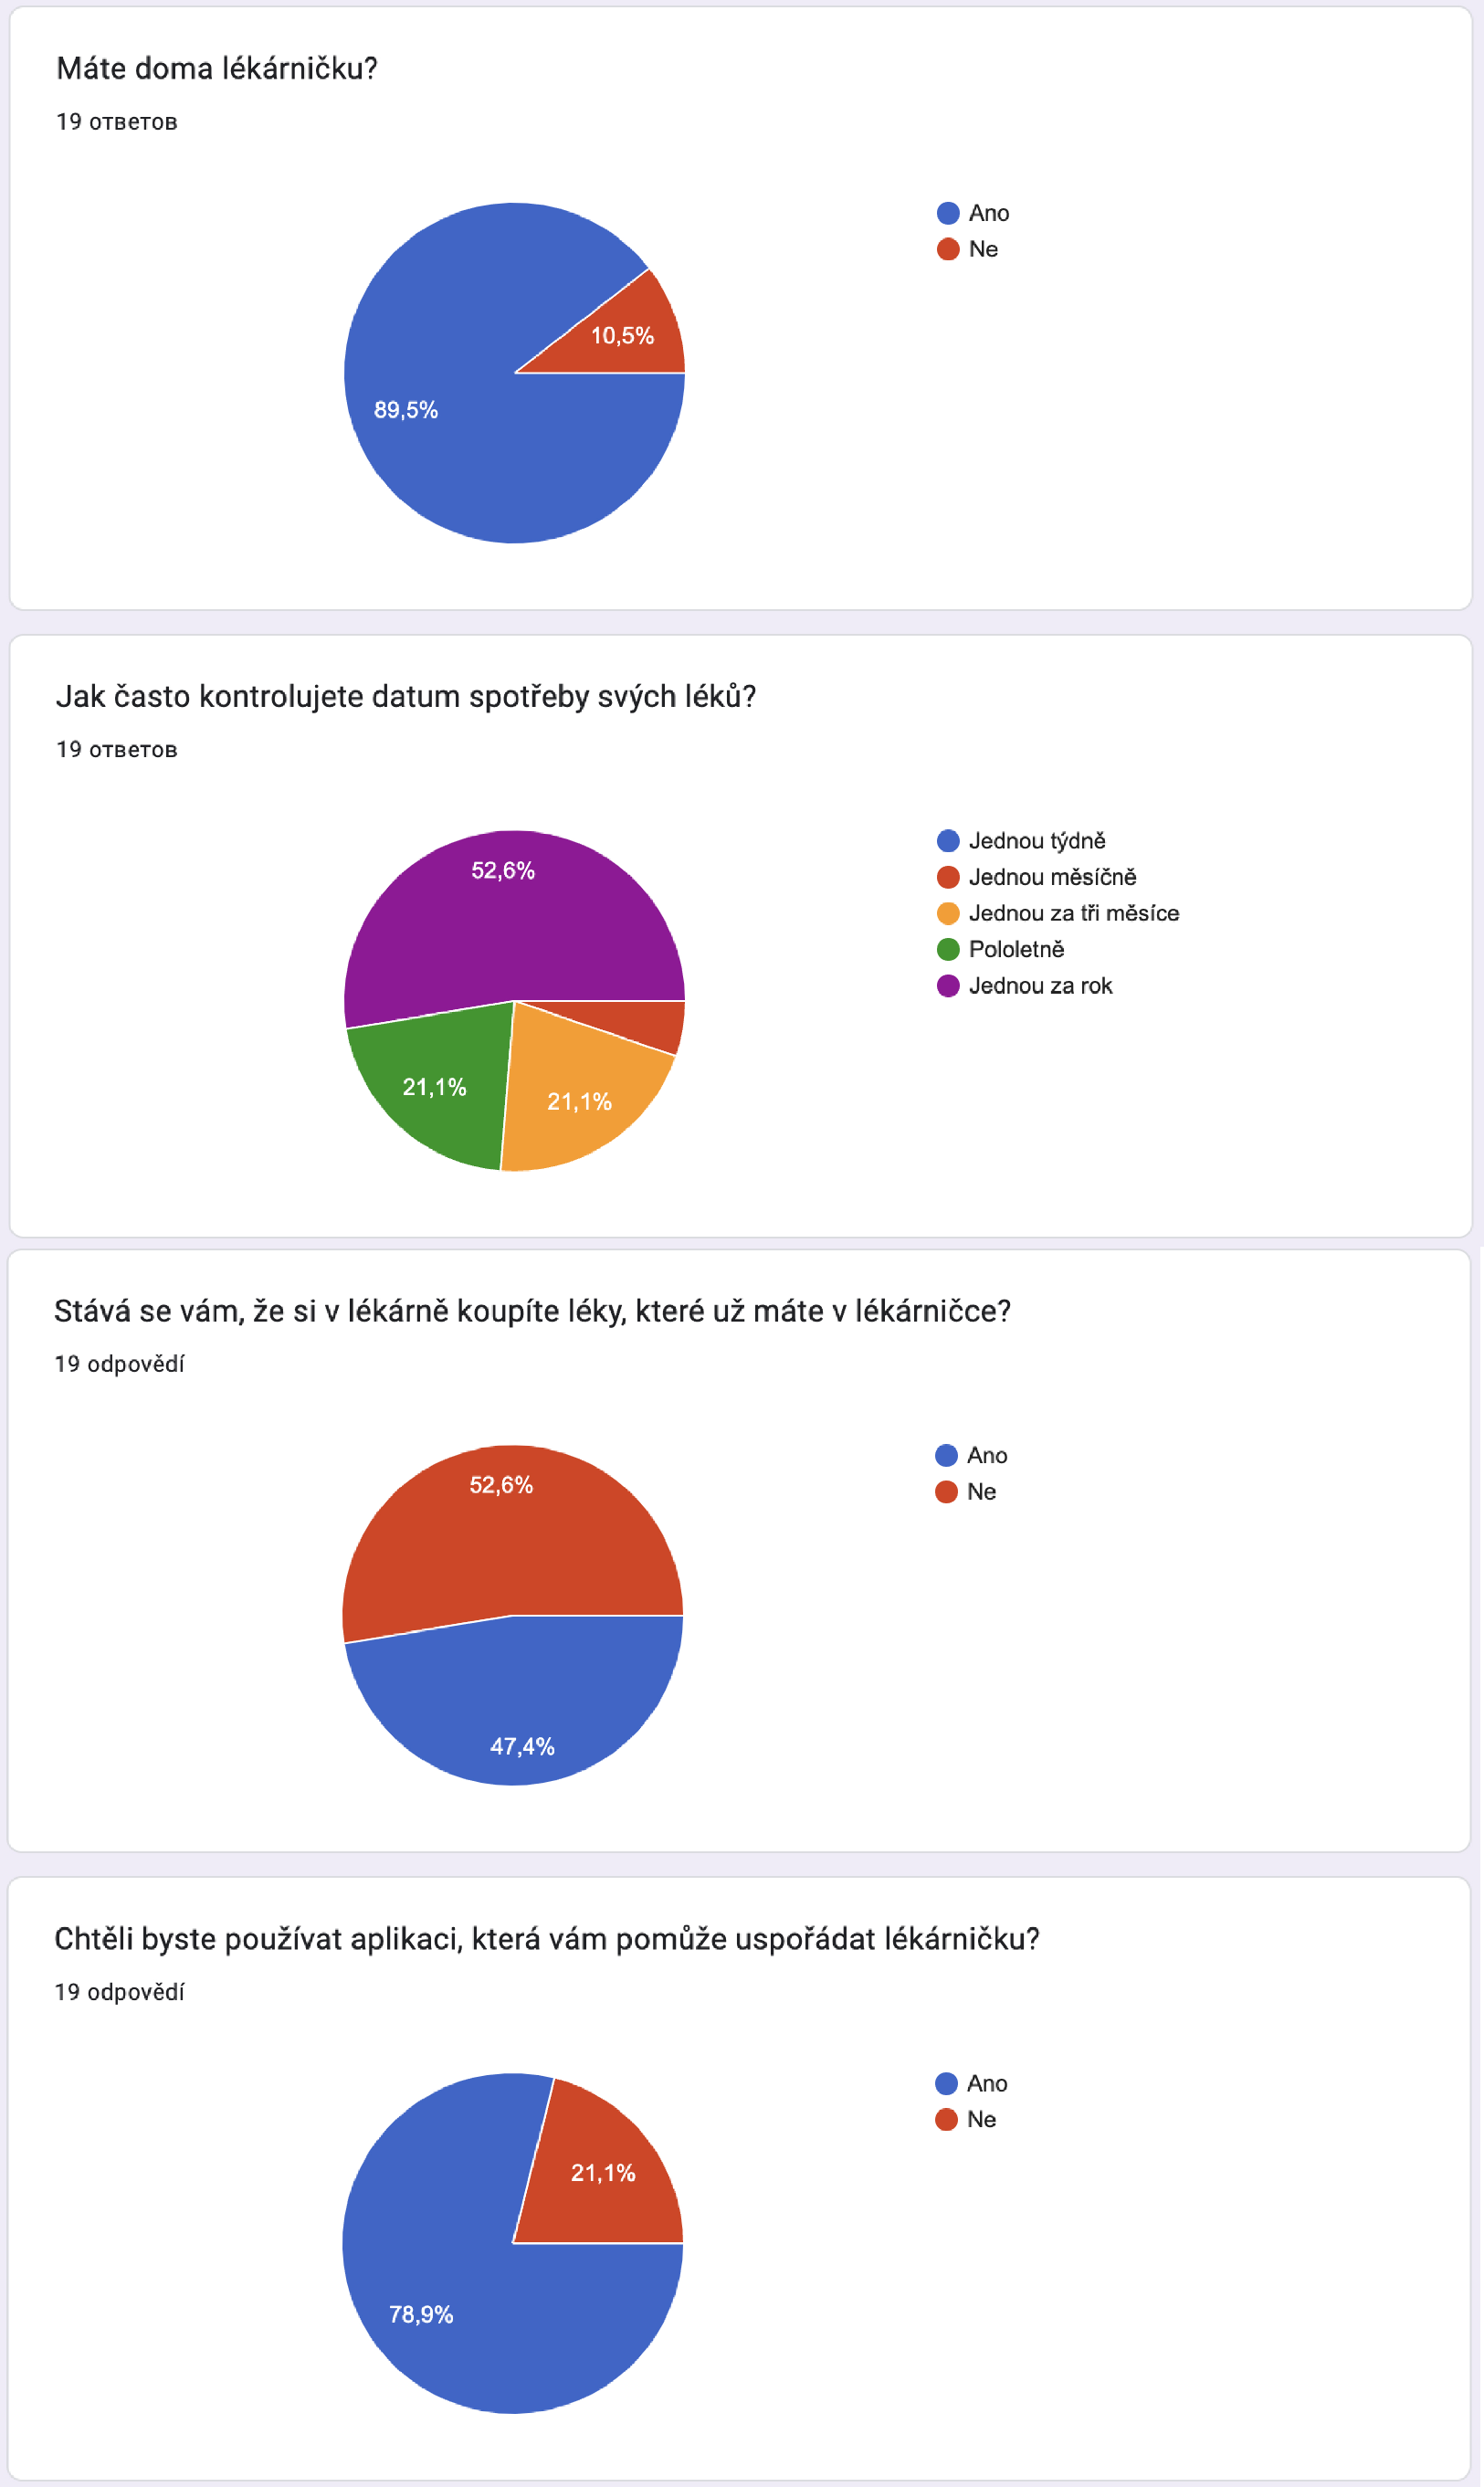
\includegraphics[width=\textwidth,height=\textheight,keepaspectratio]{Pruzkum.pdf}
		\caption{Grafické znázornění výsledků průzkumu - 1. část}
		\label{figure:pruzkum}
	\end{figure}

 \begin{figure}[!ht]
		\centering
		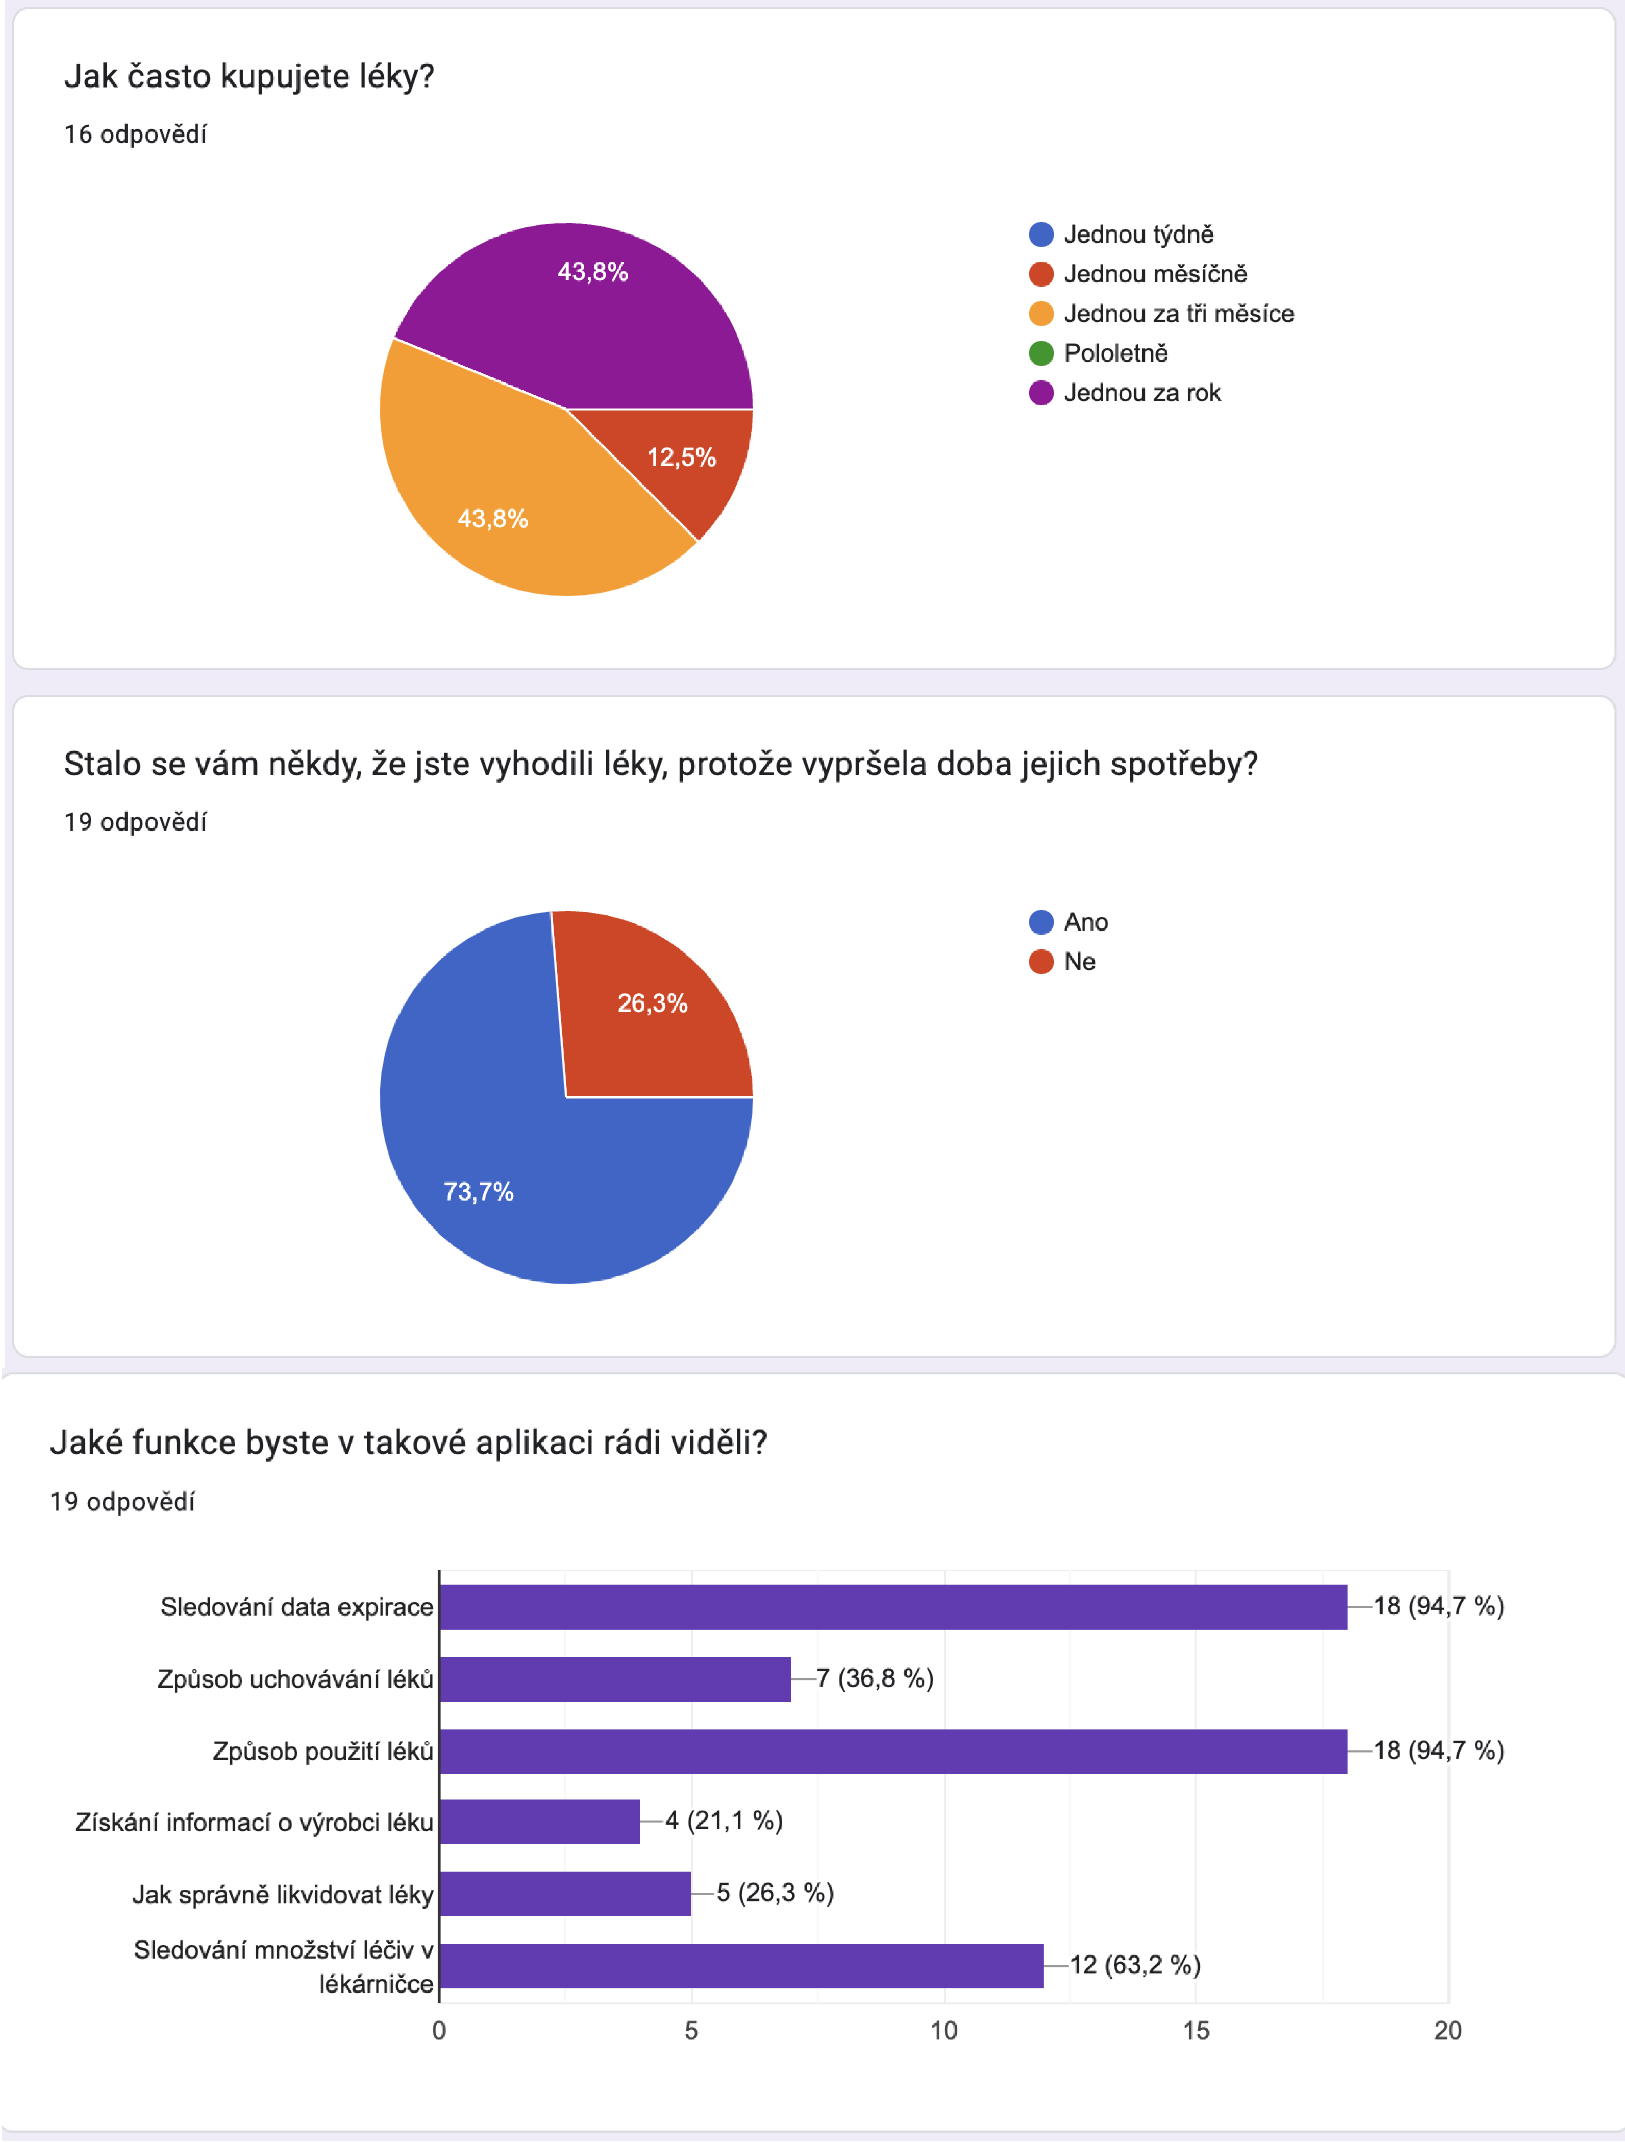
\includegraphics[width=1\linewidth]{Pruzkum1.pdf}
		\caption{Grafické znázornění výsledků průzkumu - 2. část}
		\label{figure:pruzkum1}
	\end{figure}
 \FloatBarrier

	\subsection{Existující aplikaci}
 Po provedení analýzy existujících aplikací dostupných v App Store vyšlo najevo několik společných trendů a nedostatků. Většina těchto aplikací primárně poskytuje uživatelům kalendář léků, ale postrádá komplexní sledování lékárničky. Většina těchto aplikací se navíc řídí vzorem, kdy nabízí 3denní zkušební období, po kterém se uživatelé musí přihlásit k odběru nebo provést platbu (\textbf {Figure \ref{figure:mytherapy}}).

 Jedna konkrétní aplikace, „Moje léky“, však vyniká v několika aspektech. Umožňuje uživatelům vytvářet seznamy svých léků spolu s frekvencí užívání. Navzdory tomu jsou v této aplikaci značné nedostatky. Nepodporuje sledování množství léků, neposkytuje prostředky pro přístup k návodům na užívání drog, postrádá základní oznamovací funkce a zaostává z hlediska nabídky moderního a uživatelsky přívětivého rozhraní (\textbf {Figure \ref{figure:moje leky}}).

 \begin{figure}[!ht]
		\centering	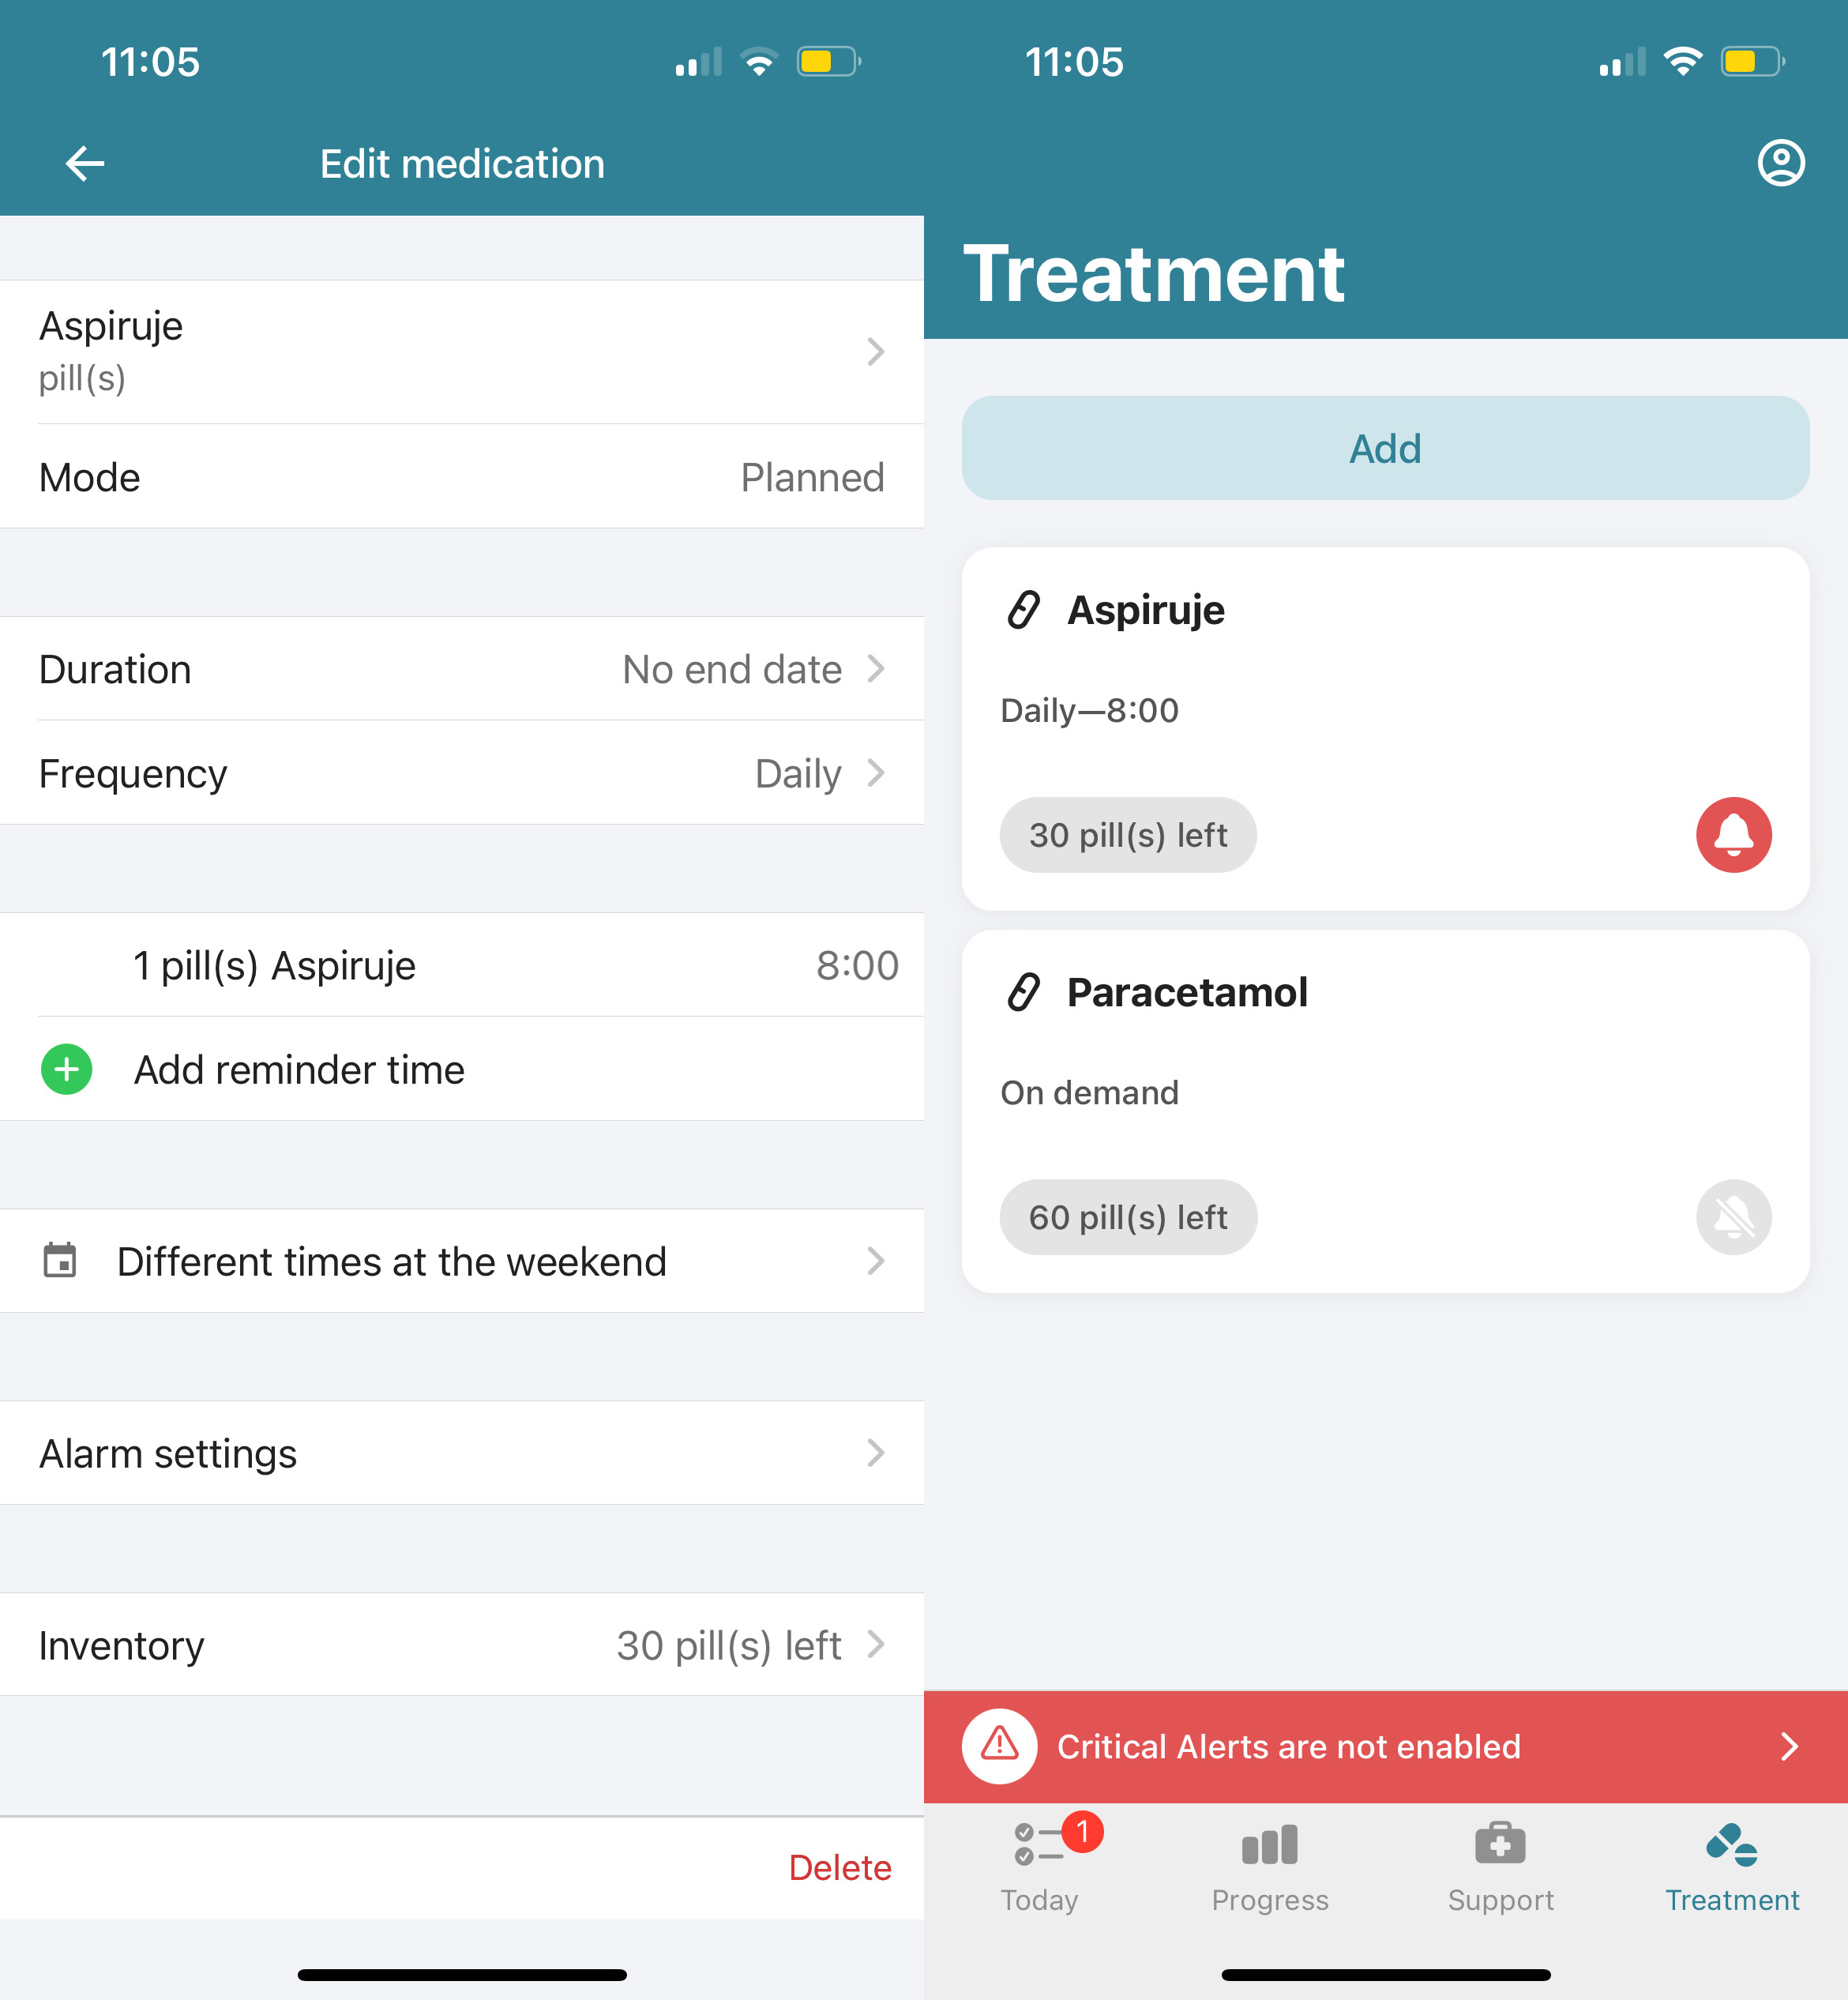
\includegraphics[width=220,height=220,keepaspectratio]{mytherapy.jpeg}
		\caption{Aplikace MyTherapy}
		\label{figure:mytherapy}
	\end{figure}
 \begin{figure}[!ht]
		\centering
		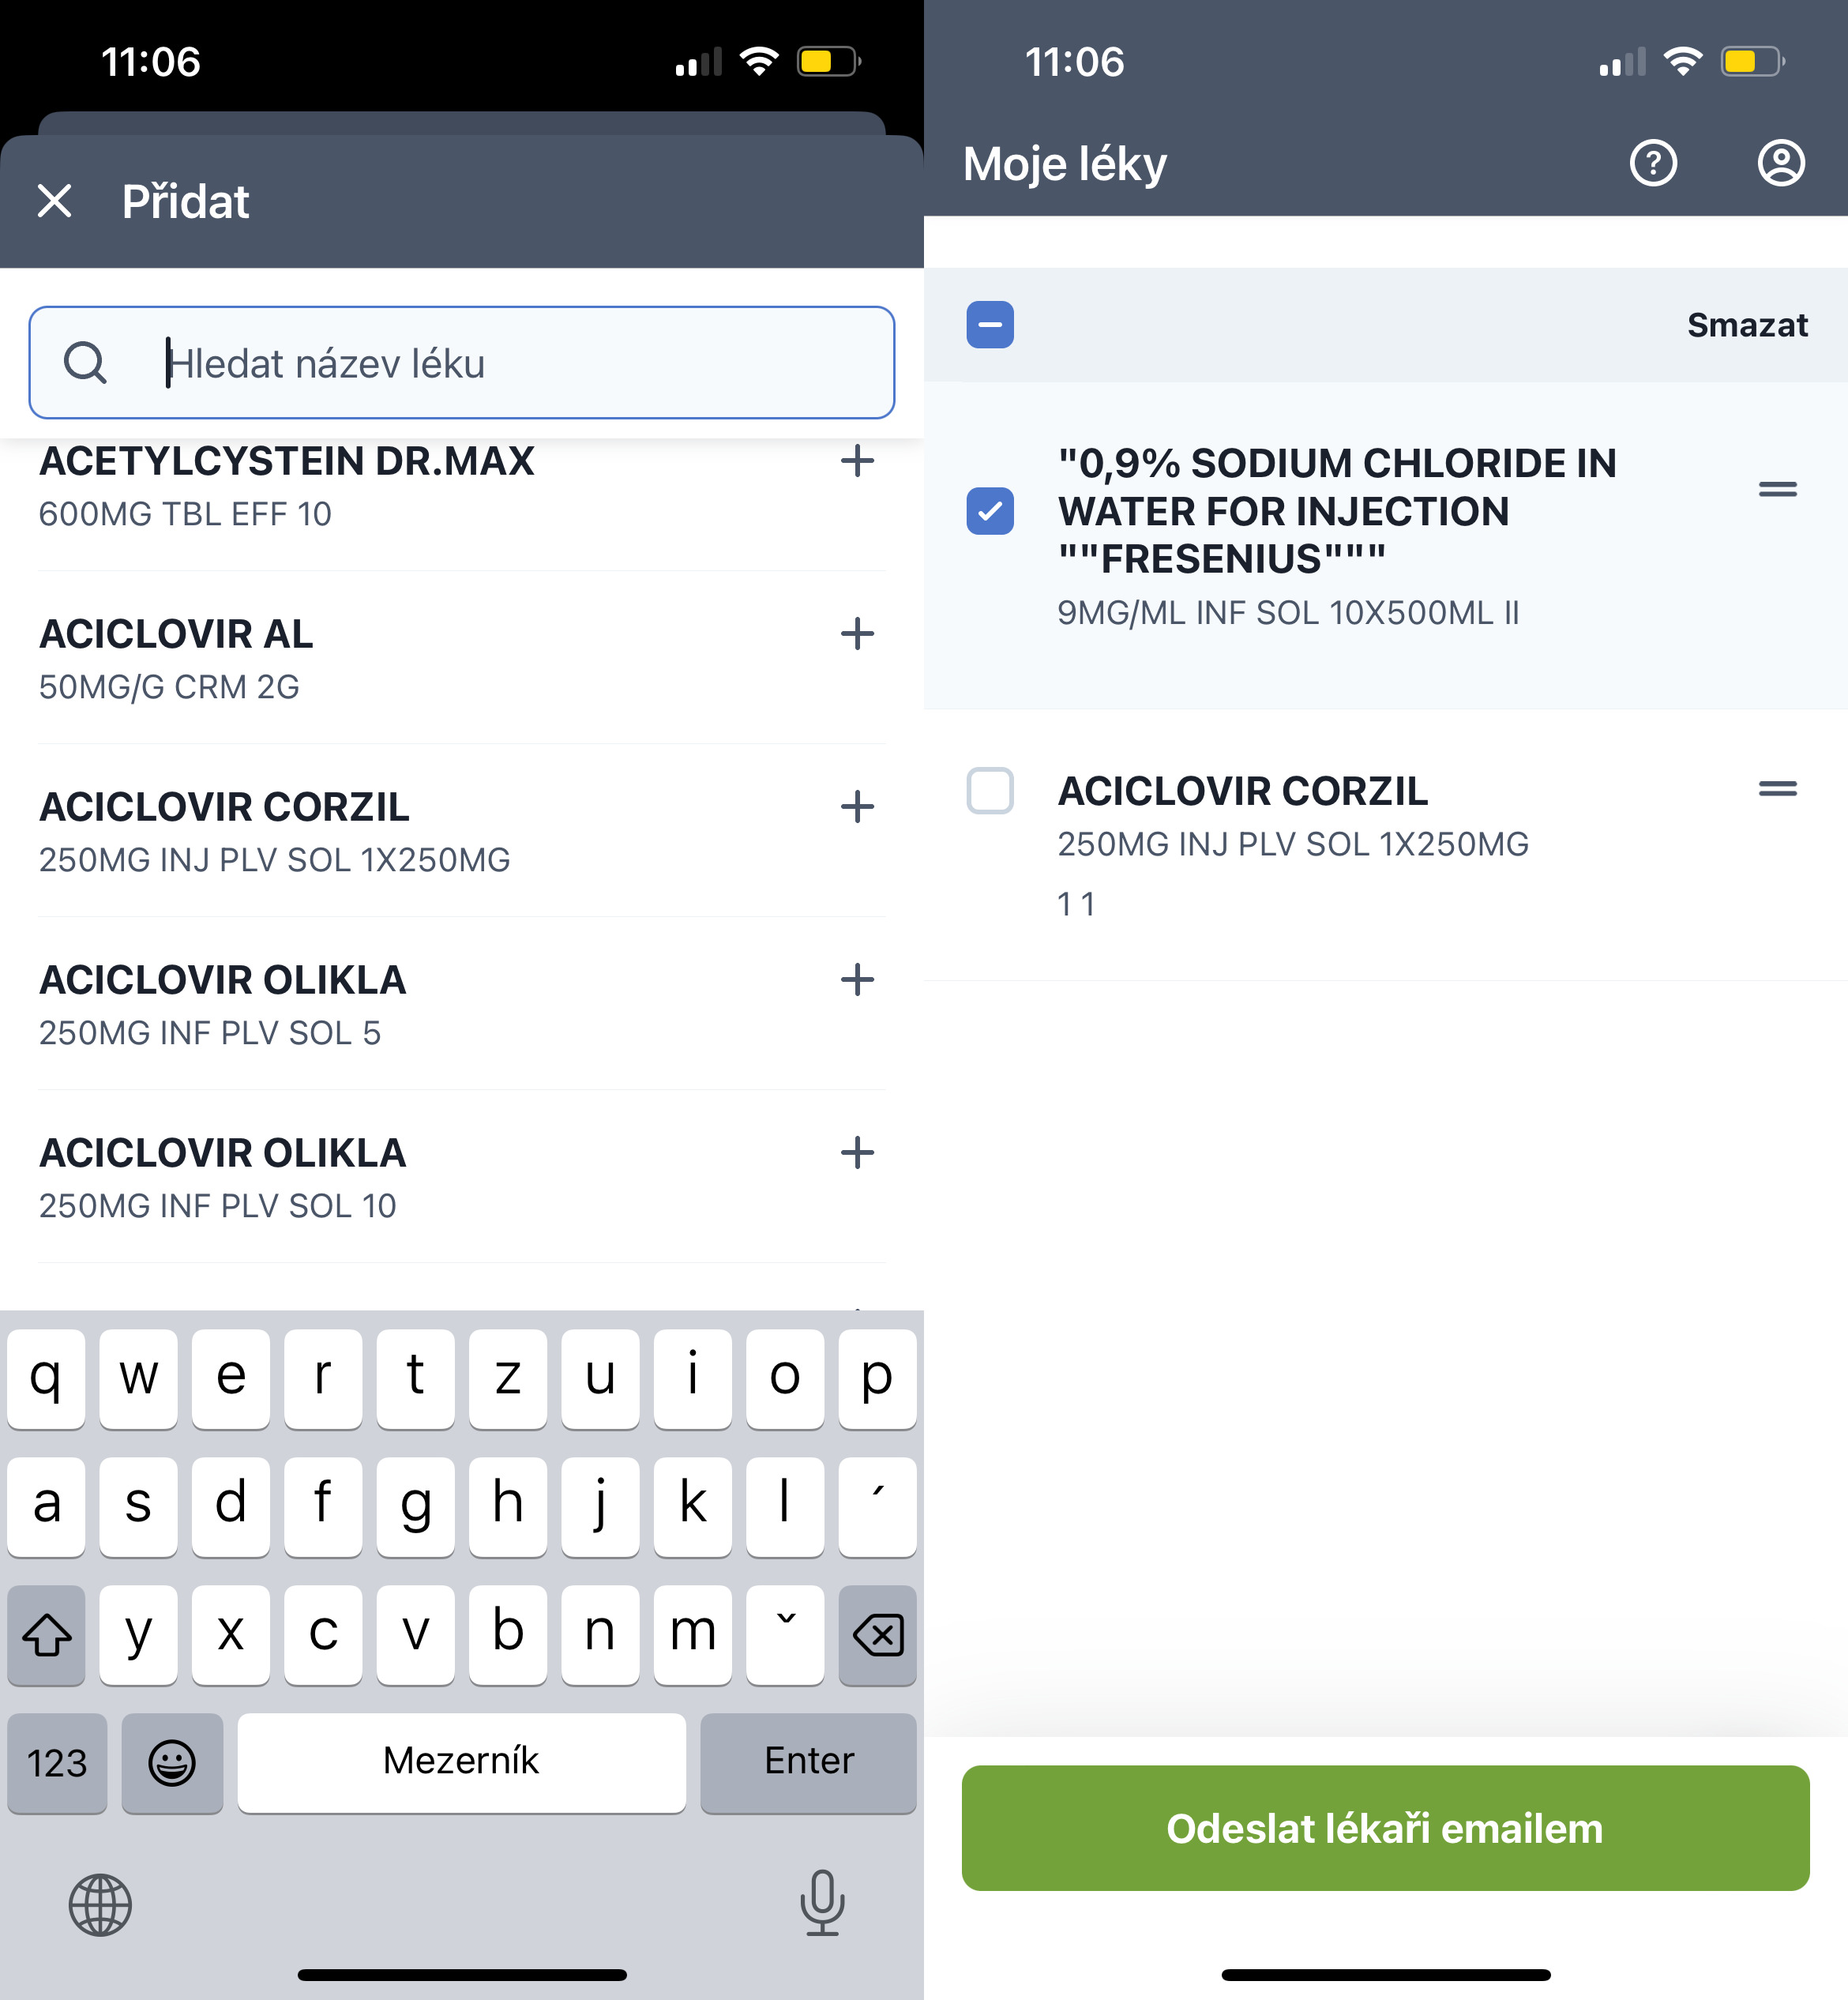
\includegraphics[width=220,height=220,keepaspectratio]{moje leky.jpeg}
		\caption{Aplikace Moje Leky}
		\label{figure:moje leky}
	\end{figure}
 \FloatBarrier

 Ve světle těchto zjištění je evidentní příležitost vytvořit vynikající aplikaci pro sledování léků, která tato omezení řeší. Taková aplikace by se mohla odlišit tím, že poskytuje následující:
 \begin{itemize}
     \item \textbf{Komplexní sledování kabinetu léků:} Na rozdíl od konkurence by naše aplikace zahrnovala robustní systém řízení zásob léků. Uživatelé budou moci nejen naplánovat své dávky léků, ale také sledovat jejich zbývající množství, což zajistí, že nikdy nečekaně nedojdou.
     \item \textbf{Úložiště informací o lécích:} Abychom uživatelům poskytli znalosti, naše aplikace by hostila rozsáhlou databázi léků. Uživatelé mohou snadno získat podrobné informace o svých lécích, jako jsou pokyny k použití, potenciální vedlejší účinky a interakce s jinými léky.
     \item \textbf{Rozhraní zaměřené na uživatele:} Uvědomujeme si důležitost uživatelské zkušenosti. Proto bude naše aplikace obsahovat elegantní, intuitivní a moderní rozhraní navržené tak, aby přidávání, úpravy a správa léků bylo snadné a zábavné.
     \item \textbf{Chytrá upozornění a připomenutí:} Naše aplikace bude uživatelům poskytovat včasné připomenutí ohledně doplňování léků a zajistí, že budou mít přehled o zásobách léků. Tato připomenutí pomohou uživatelům efektivně spravovat své léky.
 \end{itemize}
Na závěr, naše připravovaná aplikace si klade za cíl zaplnit jasnou mezeru na trhu tím, že nabídne komplexní a uživatelsky přívětivé řešení sledování léků. Odstraněním nedostatků pozorovaných ve stávajících aplikacích a upřednostněním uživatelských potřeb se snažíme poskytovat vynikající uživatelský zážitek a nástroj, který skutečně umožňuje jednotlivcům spravovat své léky efektivně a s jistotou.



	\subsection{Analýz uživatelských potřeb}
	\textbf{Klíčové potřeby uživatelů:}
 \begin{enumerate}
     \item Sledování léků: Uživatelé potřebují způsob, jak sledovat své léky, včetně léků na předpis a volně prodejných léků.
     \item Správa data expirace: Uživatelé chtějí vědět, kdy vyprší platnost jejich léků, což jim pomáhá vyhnout se užívání neúčinných nebo potenciálně škodlivých léků.
     \item Dostupnost: Uživatelé vyžadují možnost přístupu k informacím o lécích z různých míst, například doma, v autě a na cestách.
     \item Připomenutí a upozornění: Uživatelé potřebují včasné připomenutí a upozornění na náplně a na to, kdy vyprší platnost léků.
     \item Informace o lécích: Uživatelé hledají podrobné informace o každém léku, včetně pokynů k dávkování, vedlejších účinků a potenciálních interakcí s jinými léky.
     \item Soukromí a bezpečnost uživatele: Uživatelé očekávají, že informace o jejich lécích budou bezpečné a soukromé, protože se může jednat o citlivé osobní údaje.
 \end{enumerate}
\textbf{Uživatelské procesy:}
\begin{enumerate}
    \item Zadání léků: Uživatelé by měli mít možnost snadno přidat své léky do aplikace a uvést podrobnosti, jako je název léku, dávkování a množství.
    \item Sledování data expirace: Uživatelé potřebují způsob, jak zadat a sledovat data expirace svých léků, což jim umožní dostávat upozornění, když se blíží datum expirace.
    \item Vyhledávání informací o lécích: Uživatelé mohou chtít vyhledat informace o svých lécích, včetně pokynů k použití a potenciálních vedlejších účinků.
    \item Sledování na základě polohy: Uživatelé mohou potřebovat zaznamenat místo, kde uchovávají své léky, například „v autě“ nebo „doma“, aby si zajistili snadný přístup.
\end{enumerate}
Řešením těchto klíčových potřeb uživatelů a poskytováním těchto funkcí může aplikace „Lekarnicka“ pomoci lidem efektivně sledovat jejich léky a data jejich expirace na různých místech, čímž podporuje lepší řízení zdraví a dodržování léků.

    \section{Návrh aplikace}
    Rozdělení práce spočívá v tom, že každý člen týmu se specializuje na určitou část vývoje aplikace, což nakonec vede k dokončení jediné celistvé aplikace.

	\subsection{Maketa}
   krátce popište jak váš návrh řeší potřeby uživatelů (odkazujte se na
bod 5), maketu reprezentujte pomocí obrázků, diagramů nebo snímků obrazovky a
vhodného krátkého popisu.

	\subsubsection{Testování makety}

	popište použité metriky a proveďte jejich vyhodnocení, popište
testovací úlohy/scénáře, vložte informace o testovaných subjektech, popište, jak
probíhalo testování, jaké nedostatky odhalilo, a vámi navržené řešení těchto
nedostatků.

	\subsection{Architektura aplikace}

	popis architektury celé aplikace (části FE a BE*) s ohledem na
návrhový vzor MVC (nebo obdobný), popis datového modelu (datové struktury,
hlavní funkce a metody), definice API (ne všechny funkce, jen ty klíčové), seznam
vybraných technologií a nástrojů (pro FE i BE) včetně stručného zdůvodnění jejich
výběru.




\end{document}